\documentclass{article}
\usepackage{tikz, comment}
\usepackage{pifont}
\usepackage{fontspec, pgfplots}
\usetikzlibrary{arrows, decorations.markings, decorations.pathreplacing}
\begin{comment}
:Title: Not defined yet
:Tags: area using parametric equations,parametric integral formula;median of a trapezoid;arc length of a curve;perimeter;difference quotient
:Prob: 0.5758;0.5143;0.5059;0.4918;0.4881
:Author: Prof.Hu Ji-shan, HKUST
:Slug: No name yet

Description Here.........
\end{comment}
\begin{document}\centering 

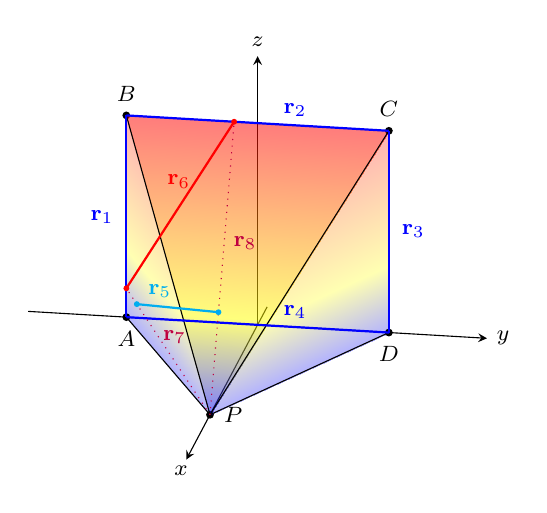
\begin{tikzpicture}[font=\footnotesize]
\pgfplotsset{compat=1.8}
\begin{axis}
[axis lines = center, view={100}{30}, scale=1, ticks=none,
axis background, xlabel = {$x$}, ylabel ={$y$}, zlabel ={$z$}, domain =-2:2, y domain =-2:2,
xmin =-200,
xmax =1499,
ymin =-699,
ymax =699,
zmin =0, 
zmax =799,
samples =10, samples y =40, z buffer = auto, 
every axis x label/.style={
    at={(ticklabel* cs:1)},
    anchor= east, xshift = 4, yshift=-4
},
every axis y label/.style={
    at={(ticklabel* cs:1)},
    anchor= west, 
},
every axis z label/.style={
    at={(ticklabel* cs:1)},
    anchor= south
}]

\addplot3[surf, shader=interp, mesh/cols=2, opacity=0.3] coordinates
		{(1000,0,0) (0,-400,0) (0,-400,600) (0,-400,600)};
\node[label={0:{$P$}},circle,fill,inner sep=1pt] at (axis cs:1000,0,0) {};
\node[label={-90:{$A$}},circle,fill,inner sep=1pt] at (axis cs:0,-400,0) {};
\node[label={90:{$B$}},circle,fill,inner sep=1pt] at (axis cs:0,-400,600) {};

\addplot3[surf, shader=interp, mesh/cols=2, opacity=0.3] coordinates
		{(1000,0,0) (0,-400,600) (0,400,600) (0,400,600)};

\addplot3[surf, shader=interp, mesh/cols=2, opacity=0.3] coordinates
		{(1000,0,0) (0, 400,0) (0,400,600) (0,400,600)};
\node[label={90:{$C$}},circle,fill,inner sep=1pt] at (axis cs:0,400,600) {};
\node[label={-90:{$D$}},circle,fill,inner sep=1pt] at (axis cs:0,400,0) {};

\addplot3[surf, shader=interp, mesh/cols=2, opacity=0.3] coordinates
		{(1000,0,0) (0, -400,600) (0,400,600) (0,400,600)};

\addplot3[surf, black] coordinates
		{(1000,0,0) (0,-400,0)};
\addplot3[surf, black] coordinates
		{(1000,0,0) (0,-400,600)};
\addplot3[surf, black] coordinates
		{(1000,0,0) (0,400,0)};
\addplot3[surf, black] coordinates
		{(1000,0,0) (0,400,600)};
				
\addplot3[surf, blue, thick] coordinates
		{(0,-400,0) (0,-400,600) (0,400,600) (0, 400, 0) (0,-400,0)};

\addplot3[surf, cyan, thick] coordinates
		{(125, -350, 75) (650, -25, 210)};

\addplot3[surf, purple, dotted] coordinates
		{(1000,0,0) (125, -350, 75) (0, -400, {600/7})};
\addplot3[surf, purple, dotted] coordinates
		{(1000,0,0) (650, -25, 210) (0, {-500/7}, 600)};

\addplot3[surf, red, thick] coordinates
		{(0, -400, {600/7}) (0, {-500/7}, 600)};

\node[label={180:{}},circle, cyan, fill, inner sep= 0.75pt] at (axis cs:125,-350,75) {};
\node[label={180:{}},circle, cyan, fill,inner sep= 0.75pt] at (axis cs:650,-25,210) {};
\node[label={180:{}},circle, red, fill,inner sep= 0.75pt] at (axis cs:0, -400, 85.7143) {};
\node[label={180:{}},circle, red, fill,inner sep= 0.75pt] at (axis cs: 0, -71.4286, 600) {};

\node[label={180:{\color{blue} ${\bf r}_1$}}] at (axis cs:0,-380,300) {};
\node[label={20:{\color{blue} ${\bf r}_2$}}] at (axis cs:0,20,580) {};
\node[label={0:{\color{blue} ${\bf r}_3$}}] at (axis cs:0,380,300) {};
\node[label={20:{\color{blue} ${\bf r}_4$}}] at (axis cs:0,20,-20) {};

\node[label={90:{\color{cyan} ${\bf r}_5$}}] at (axis cs:400,-240,115) {};
\node[label={90:{\color{red} ${\bf r}_6$}}] at (axis cs:0,-240,335) {};

\node[label={40:{\color{purple} ${\bf r}_7$}}] at (axis cs:500,-275,10) {};
\node[label={40:{\color{purple} ${\bf r}_8$}}] at (axis cs:500,-60,300) {};

\end{axis}

\end{tikzpicture}
\end{document}